% Requested

O problema de decisão Gold Star consiste em resolver um sistema de 5 equações da forma
\begin{equation}
\systeme*{
A \_ B = D \_ E ,
G \_ F = D \_ C ,
I \_ H = F \_ E ,
G \_ H = J \_ A ,
I \_ J = B \_ C
}
\end{equation}
Sendo \_ possível de ser substituído por um dos seguintes operadores:
\begin{equation}
    +\  -\  \mbox{×}\ \ \mbox{÷}
\end{equation}

Entre as 5 equações, apenas são partilhadas 10 variáveis para ser possível formar um padrão em forma de estrela ao dispor as equações como na figura \ref{fig: gold_star_example}.

\begin{figure}[ht]
\centering
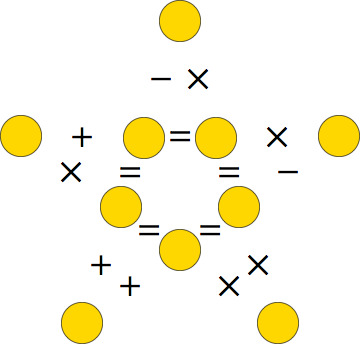
\includegraphics[width=0.3\textwidth]{figuras/template.jpg}
\caption{5 equações dispostas em padrão de forma estrela}
\label{fig: gold_star_example}
\end{figure}

Para obter uma solução válida, apenas podem ser usados os números inteiros de 0 até 9 e cada dígito só pode ser usado uma vez. Para além disso, os resultados de cada lado da equação não podem resultar em números não inteiros.